\section{How many siblings?}
To find the Lot of the Number of Siblings\footnote{Note that \textsl{siblings} is being used here and elsewhere in place of \textsl{brothers}.}, count (in the order of the signs) from \Mercury\, to \Jupiter\, (by night, from \Jupiter\, to \Mercury) and add the difference to the Ascendant. The number of planets aspecting the place of the lot gives you the number of siblings.

Indications from the planets aspecting the place are:
\begin{description}[labelindent=0em , labelwidth=6em, labelsep=0.5em, leftmargin =!]
\item [\Venus,\Mercury] in aspect from a good place, from feminine signs indicates sisters; in masculine signs, brothers

\item[\Saturn,\Mars,\Sun\,\Moon] peregrine, indicate the loss of siblings but if in their own places his siblings ``will not love him and are not his friends or who have no use for him because what the malefics indicate is not complete''

\item[any planet] in aspect from a bad place indicates the siblings ``have no good in them or have sicknesses, or that there is enmity between them, and bad and evil [are their] opinion and thought [of each other]
\end{description}

\subsection{Indications from the 3rd Place}
If the sign on the 3rd place is double-bodied (\Gemini, \Virgo, \Sagittarius, \Pisces) or its lord is in a double-bodied sign then the siblings are not the children of both parents.

Indications from the planets as to birth-order:
\begin{itemize}
\item[\Saturn,\Mars] older brothers
\item[\Jupiter,\Mars] middling brothers
\item[\Mercury] younger brothers
\item[\Moon] older sisters
\item[\Venus] younger sisters
\end{itemize}

\subsection{General Indications from Mars}
If the 1st and 2nd triplicity rulers of \Mars\, are in bad places, it indicates a small number of siblings.

If one triplicity ruler is in  a good place and the other in a bad place then the person has siblings ``but it is inevitable that he will see their death.''

\vspace{-1em}
\begin{figure}[H]
\centering
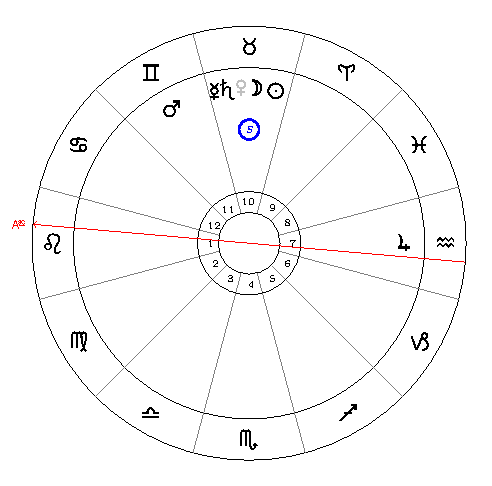
\includegraphics[width=0.7\textwidth]{charts/1_01}
\vspace{-1em}
\caption{Chart 01: Man with 5 Siblings}
\end{figure}

The chart of a man with the \Sun, \Moon, \Saturn, \Mercury\footnote{\Venus\, is missing from the original chart, Dykes places it in the 10th, dating the chart to May 2 or 3, 29 AD JC, $\approx$ 11:30AM Sidon, Lebanon.}, and the Lot of Siblings in the Midheaven in Taurus with \Mars\, in \Gemini, \Jupiter\, in \Aquarius, and the Ascendant in \Leo.

\Saturn\, and \Mercury\, are the indicators of siblings as they are the triplicity rulers of \Mars\, (the general indicator of siblings). ``Because they both happen to be above the earth you count from them to the ascendent, but if they were below the earth you would count from the ascendent to them.''

Predict the person will have five siblings as the two triplicity rulers are in \Taurus\, and counting from there to the ascendent sign of \Leo\, gives: \Taurus\, (1) + \Gemini\, (double-bodied gives 2) + \Cancer\, (1) + \Leo\, (1) = 5.

If both the triplicity rulers had not been in one sign it would be necessary to take the count from whichever was eastern and in a strong place, or, if both were of equal strength, to start the count from the day or night triplicity ruler (depending on the chart sect). 

The Lot of Siblings is in a feminine sign (\Taurus) with \Saturn\, indicating his sister will die, as will both an older and his youngest brothers because the \Sun\, and \Mercury\, are also with the lot and \Saturn\, in \Taurus\, but the fullest effect of these will not be felt because \Jupiter\, aspects the place\footnote{An example of the \Square\, of \Jupiter\, being beneficial rather than harmful when he is angular and in one of his own places (he's the participting triplicity ruler of \Aquarius).}